\documentclass[a4paper, 12pt]{article}%тип документа

%отступы
\usepackage[left=2cm,right=2cm,top=2cm,bottom=3cm,bindingoffset=0cm]{geometry}
\setlength{\parindent}{5ex}

%Русский язык
\usepackage[T2A]{fontenc} %кодировка
\usepackage[utf8]{inputenc} %кодировка исходного кода
\usepackage[english,russian]{babel} %локализация и переносы

%Вставка картинок
\usepackage{graphicx}
\graphicspath{{pictures/}}
\DeclareGraphicsExtensions{.pdf,.png,.jpg}

%Графики
\usepackage{pgfplots}
\pgfplotsset{compat=1.9}

%Математика
\usepackage{amsmath, amsfonts, amssymb, amsthm, mathtools}

%Таблицы
\usepackage{longtable} 
\usepackage{float}

%Римские цифры
\newcommand{\RomanNumeralCaps}[1]{\uppercase\expandafter{\romannumeral#1}}

\usepackage{multirow}


\begin{document}
	\begin{titlepage}
		\begin{center}
			\textsc{Федеральное государственное автономное образовательное учреждение высшего образования«Московский физико-технический институт (национальный исследовательский университет)»\\[5mm]
			}
			
			\vfill
			
			\textbf{Отчет по лабораторной работе 2.4.1 \\[3mm]
				Определение теплоты испарения жидкости.
				\\[50mm]
			}
			
		\end{center}
		
		\hfill
		\begin{minipage}{.5\textwidth}
			Выполнил студент:\\[2mm]
			Сериков Василий Романович\\[2mm]
			группа: Б03-102\\[5mm]
			
		\end{minipage}
		\vfill
		\begin{center}
			Москва, 2022 г.
		\end{center}
		
	\end{titlepage}
	
	\newpage
	\textbf{Аннотация}\\
	
	
	\textbf{Цель работы: }\\


     1)Измерение давления насыщенного пара жидкости при разной температуре 2) Вычисление по полученным данным теплоты испарения с помощью уравнения Клапейрона–Клаузиуса.\\
	
	
	\textbf{Теоретические сведения: } \\
	
	
	Испарением называется переход вещества из жидкого в газообразное состояние. Оно происходит на свободной поверхности жидкости. При испарении с поверхности вылетают молекулы, образуя над ней пар. Для выхода из жидкости молекулы должны преодолеть силы молекулярного сцепления. Кроме того, при испарении совершается работа против внешнего давления $ P $, поскольку объем жидкости меньше объема пара. Не все молекулы жидкости способны совершить эту работу, а только те из них, которые обладают достаточной кинетической энергией. Поэтому переход части молекул в пар приводит к обеднению жидкости быстрыми молекулами, т.е. к ее охлаждению. Чтобы испарение проходило без изменения температуры, к жидкости нужно подводить тепло. Количество теплоты, необходимое для изотермического испарения одного моля жидкости при внешнем давлении, равном упругости ее насыщенных паров, называется молярной теплотой испарения (парообразования).
	
	Теплоту парообразования жидкостей можно измерить непосредственно при помощи калориметра. Такой метод, однако, не позволяет получить точных результатов из-за неконтролируемых потерь тепла, которые трудно сделать малыми. В настоящей работе для определения теплоты испарения применен косвенный метод, основанный на формуле Клапейрона–Клаузиуса:
	
	\begin{equation}\label{Kl-Kl}
		\frac{dP}{dT}=\frac{L}{T\left(V_2-V_1\right)}.
	\end{equation}
	
	Здесь $ P $ -- давление насыщенного пара жидкости при температуре $ T $, $ T $ -- абсолютная температура жидкости и пара, $ L $ -- теплота испарения жидкости, $ V_2 $ -- объем пара, $ V_1 $ -- объем жидкости. Найдя из опыта $ dP/dT $, $ T $, $ V_2 $ и $ V_1 $, можно определить $ L $ путем расчета. Величины $ L $, $ V_2 $ и $ V_1 $ в формуле \eqref{Kl-Kl} должны относиться к одному и тому же количеству вещества; мы будем относить их к одному молю.
	
	В нашем приборе измерения производятся при давлениях ниже атмосферного. В этом случае задача существенно упрощается.
	
	При нашей точности опытов величиной $ V_1 $ в \eqref{Kl-Kl} можно пренебречь.
	
	Обратимся теперь к $ V_2 $, которое в дальнейшем будем обозначать просто $ V $. Объем $ V $ связан с давлением и температурой уравнением Ван-дер-Ваальса:
	
	\begin{equation}\label{VDV}
		\left(P+\frac{a}{V^2}\right)\left(V-b\right)=RT.
	\end{equation}
	
	Из табличных данных следует, что $ b $ одного порядка с $ V_1 $. В уравнении Ван-дер-Ваальса величиной $ b $ следует пренебречь. Пренебрежение членом $ a/V^2 $ по сравнению с $ P $ вносит ошибку менее 3\%. При давлении ниже атмосферного ошибки становятся еще меньше. Таким образом, при давлениях ниже атмосферного уравнение Ван-дер-Ваальса для насыщенного пара мало отличается от уравнения Клапейрона. Положим поэтому
	
	\begin{equation}\label{Volume}
		V=\frac{RT}{P}.
	\end{equation}
	
	Подставляя \eqref{Volume} в \eqref{Kl-Kl}, пренебрегая $ V_1 $ и разрешая уравнение относительно $ L $, найдем
	
	\begin{equation}\label{final}
		L=\frac{RT^2}{P}\frac{dP}{dT}=-R\frac{d(\ln P)}{d(1/T)}.
	\end{equation}
	
	В нашем опыте температура жидкости измеряется термометром, давление пара определяется при помощи манометра, а производные $ dP/dT $ или $ d(\ln P)/d(1/T) $ находятся графически как угловой коэффициент касательной к кривой $ P(T) $ или соответственно к кривой, у которой по оси абсцисс отложено $ 1/T $, а по оси ординат $ \ln P $.\\
	
    \textbf{Экспериментальная установка}\\
	
	\begin{figure}[H]
		\center{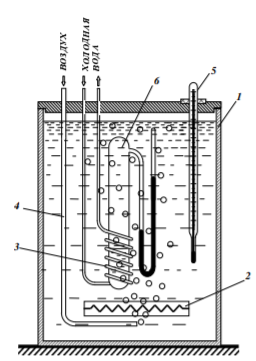
\includegraphics [scale=1]{photo 1.png}}
		\caption{Схема установки для определения теплоты испарения.}
	\end{figure}

	Схема установки изображена на рисунке 1. Наполненный водой резервуар 1 играет роль термостата. Нагревание термостата производится спиралью 2, подогреваемой электрическим током. Для охлаждения воды в термостате через змеевик 3 пропускается водопроводная вода. Вода в термостате перемешивается воздухом, поступающим через трубку 4. Температура воды измеряется термометром 5. В термостат погружен запаянный прибор 6 с исследуемой жидкостью. Над ней находится насыщенный пар (перед заполнением прибора воздух из него был откачан). Давление насыщенного пара определяется по ртутному манометру, соединенному с исследуемым объемом. Отсчет показаний манометра производится при помощи микроскопа.
	
	На рисунке \ref{img2} приведена более полная схема такой же установки, но с использованием современного термостата. Установка включает термостат A, экспериментальный прибор B и отсчетный микроскоп C.
	
	Экспериментальный прибор B представляет собой емкость 12, заполненную водой. В нее погружен запаянный прибор 13 с исследуемой жидкостью 14. Перед заполнением исследуемой жидкости воздух из запаянного прибора был удален, так что над жидкостью находится только её насыщенный пар. Давление пара определяется по ртутному манометру 15, соединенному с емкостью 13. Численная величина давления измеряется по разности показаний отсчетного микроскопа 16, настраиваемого последовательно на нижний и верхний уровни столбика ртути манометра. Показания микроскопа снимаются по шкале 17.
	
	Описание прибора указывает на второе важное преимущество предложенного косвенного метода измерения $ L $ перед прямым. При непосредственном измерении теплоты испарения опыты нужно производить при неизменном давлении, и прибор не может быть запаян. При этом невозможно обеспечить такую чистоту и неизменность экспериментальных условий, как при нашей постановке опыта.
	
	Описываемый прибор обладает важным недостатком: термометр определяет температуру термостата, а не исследуемой жидкости (или ее пара). Эти температуры близки друг к другу лишь в том случае, если нагревание происходит достаточно медленно. Убедиться в том, что темп нагревания не является слишком быстрым, можно, сравнивая результаты, полученные при нагревании и при остывании прибора. Такое сравнение необходимо сделать. Для ориентировки укажем, что температуру воды в калориметре следует менять не быстрее, чем на 1 $ ^\circ C $ в течение 1–3 минут.
	\begin{figure}[H]
		\center{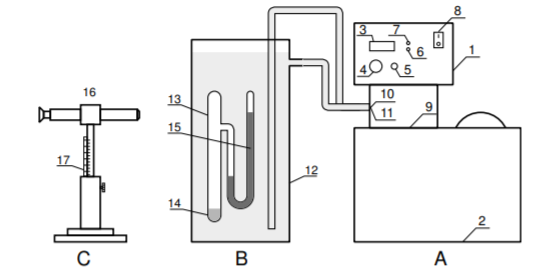
\includegraphics [scale=1]{photo 2.png}}
		\caption{Схема установки для определения теплоты испарения.}
	\end{figure}
	
	\textbf{В работе используются:}\\
	
	Термостат; герметический сосуд, заполненный исследуемой жидкостью; отсчетный микроскоп.\\
	
	
	\textbf{Результаты измерений и обработка данных: }
	\begin{enumerate}
	\item Измерим разность уровней$\Delta h $ в ртутном $U $ - образном манометре с помощью микроскопа и температуру по индикаторному табло. Полученные результаты занесем в таблицу ($\Delta P = \rho_{\text{ртуть}} g \Delta h $).
	
	\begin{longtable}{|c|c|c|}
		\hline
		T, $^\circ C$ & $\Delta h$, мм & $\Delta P$, Па \\ \hline
		20 & 17,4 & 2365 \\ \hline
		21 & 18,1 & 2461\\ \hline
		22 & 19,45 & 2644 \\ \hline
		23 & 20,45 & 2780 \\ \hline
		24 & 21,8 & 2964 \\ \hline
		25 & 23,1 & 3141 \\ \hline
		26 & 24,65 & 3351 \\ \hline
		27 & 26,25 & 3569 \\ \hline
		28 & 27,75 & 3773 \\ \hline
		29 & 29,1 & 3956 \\ \hline
		30 & 30.9 & 4201 \\ \hline
		31 & 32,85 & 4466 \\ \hline
		32 & 34,5 & 4691 \\ \hline
		33 & 36,5 & 4963 \\ \hline
		34 & 38,5 & 5235 \\ \hline
		35 & 40,4 & 5493 \\ \hline
		36 & 42,25 & 5744 \\ \hline
		37 & 45 & 6118 \\ \hline
		38 & 47,15 & 6410 \\ \hline
		39 & 49,7 & 6757\\ \hline
		40 & 52,5 & 7138\\ \hline
		\caption{Полученные данные}
	\end{longtable}
	\item Построим графики в координатах $T, P$ и в координатах $1/T, \ln P$
	
	\begin{figure}[H]
		\center{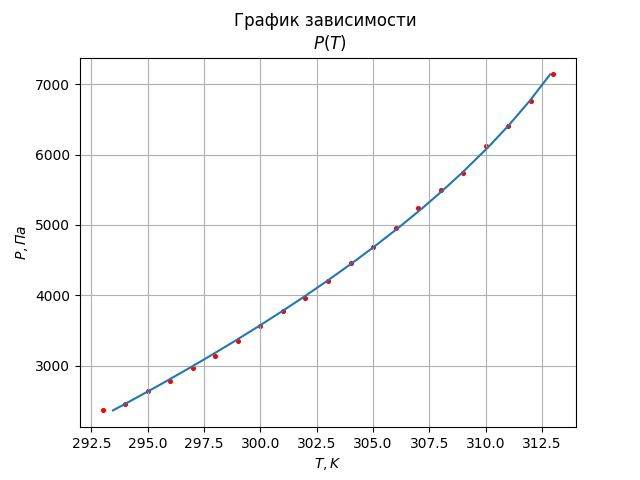
\includegraphics [scale=1]{P(T).png}}
	\end{figure}
	
	\begin{figure}[H]
		\center{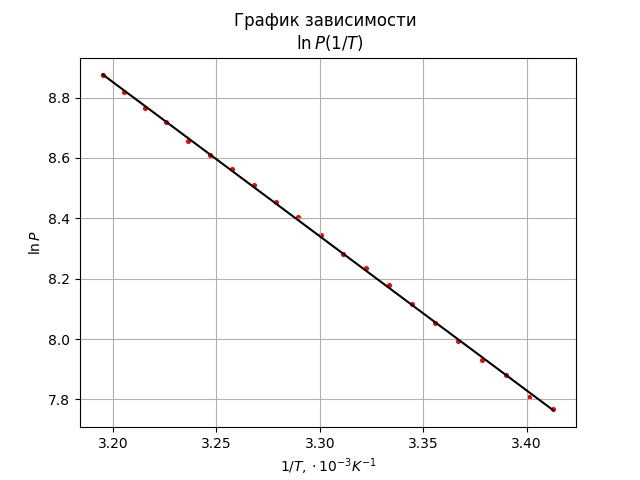
\includegraphics [scale=1]{ln P(T-1).png}}
	\end{figure}
	
	\item Вычислим $L$, пользуясь данными полученными из графика $T(P)$.
	
	Аппроксимируем по МНК функцией вида:
	 \[ P=\alpha \exp^{\beta T}  => \ln P = \beta T + \ln \alpha\]
	
	\[ \beta = \frac{\langle \ln P \cdot T \rangle - \langle T \rangle \langle \ln P \rangle}{\langle T^2 \rangle - \langle T \rangle ^2},\]
	\[ \ln \alpha = \langle \ln P \rangle - \beta\langle T \rangle. \]
	
	
	Получим: 
	
	$\alpha = 1,4 \pm 0,2 \cdot 10^{-4} $ Па, 
	
	$\beta = 5,6 \pm 0,1 \cdot 10^{-2} K^{-1}$ 
	
	
	\item По полученным коэффициентам вычислим теплоту парообразования воды:
	
	$$
	\frac{dP}{dT} = \alpha \beta e^{\beta T}.
    $$
    Подставляя, получаем:
    $$
    L=\frac{RT^2\alpha \beta }{P}e^{\beta T}.
    $$
	
	
	\item По полученной формуле подсчитаем $L$ для каждой температуры, полученные данные занесем в таблицу. ($\varepsilon_L \approx 13 \% $ )
	
	\begin{longtable}{|c|c|c|c|c|c|c|c|c|c|c|c|}
		\hline
	T, K& 293& 294& 295&296& 297& 298& 299& 300& 301& 302&303  \\ \hline
	L, Дж/г & 2237& 2291& 2272&2302 & 2301& 2314& 2310& 2311& 2329& 2366& 2374 \\ \hline
	\end{longtable}
	
		\begin{longtable}{|c|c|c|c|c|c|c|c|c|c|c|}\hline
		T, K& 304& 305& 306& 307& 308& 309& 310& 311& 312& 313   \\ \hline
		L, Дж/г & 2379& 2413& 2429& 2453& 2490& 2537& 2537& 2579& 2606& 2627  \\ \hline
		\caption{Полученная теплота парообразования}
	\end{longtable}
	
	
	\item Теперь получим теплоту парообразования из 2-го графика. Коэффициент наклона прямой - искомая производная:
	$$ L =-R\frac{d(\ln P)}{d(1/T)}  => L = -R k$$
	 где к = - 5104 $\pm 223$ К - найдено по МНК.
	\item Получим L = 2356 $\pm 103 $ Дж/г\\
	
	
	
	\textbf{Обсуждение результатов: }\\
	
	В ходе данной работы мы изучали явление парообразования воды и получали зависимость давления насыщенного пара от температуры. Обработав полученные данные двумя способами, мы получили следующие теплоты парообразования воды:
	$\overline L_1 = 2432 \pm 316$ Дж/г - получено по графику $P(T)$,
	$L_2 = 2356 \pm 103$ Дж/г - получено по графику  $\ln P(1/T)$.
	 Можно заметить, что второй результат более точный и ближе находится к табличному значению ($L_{\text{табл}}$ = 2259 Дж/г)
	
	
	\textbf{Выводы: }\\
	В данной работе мы определили теплоту парообразования воды и, обрабатывая данные двумя способами, получили значения совпадающие с табличным в пределах погрешности.
	
	
	\end{enumerate}
	\end{document}